\documentclass[8]{article}
\usepackage[utf8]{inputenc}
\usepackage{physics}
\usepackage{listings}
\usepackage{graphicx}
\usepackage{flexisym}

\title{Bio-Mathematics 214 HomeWork}
\author{Bhekimpilo Ndhlela (18998712)}

\date{09 April 2018}

\begin{document}

\maketitle
\section*{Question}
\textbf{\\$ln(\frac{u^\lambda}{v}) + u - v = k$\\ $ln(\frac{u^\lambda}{v}) + u - v  - k = 0$\\
This is an implicit function in $u$ and $v$. However, we can plot the solution curves on the u, v plane for various values of $k$ and $\lambda$ . Note: That $\lambda$ can be negative.\\ \\
Plot the solution curves for the implicit solution above using any programming language.
}

\pagebreak
\subsection*{Python Source Code:}
\begin{lstlisting}[language=Python]
#!/usr/bin/python
def solution(e, k):
    f = lambda u, v : (ln(u**e) / v) + u - v - k
    u = linspace(1., 20., 1000)
    v = linspace(1., 20., 1000)

    f_vals = [f(x,y) for x,y in zip(u,v)]
    plot_implicit_solution(u,v, f_vals)

def plot_implicit_solution(u,v, f_vals):
    plt.plot(u, f_vals, "k-", label="f(u)")
    plt.plot(v, f_vals, "r-", label="f(v)")
    plt.title("IMPLICIT SOLUTIOIN CURVE")
    plt.xlabel("v")
    plt.ylabel("u")
    plt.legend(bbox_to_anchor=(.65, .9))
    plt.show()

if __name__ == "__main__":
    import matplotlib.pyplot as plt
    from sys import (argv, exit)
    from math import log as ln
    from numpy import linspace

    if len(argv) == 3:
        solution(int(argv[1]), int(argv[2]))
    else:
        exit("USAGE: solution.py <lambda> <k>")

else:
    from sys import exit
    exit("USAGE: solution.py <lambda> <k>")

\end{lstlisting}

\pagebreak
\begin{figure}[h!]
  \centering
  \begin{subfigure}{\linewidth}
    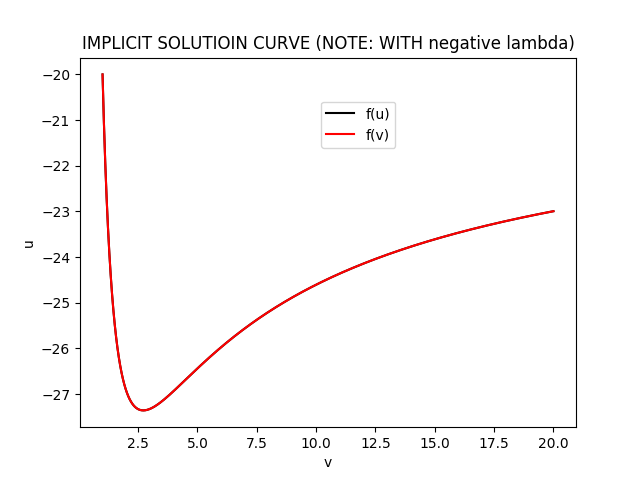
\includegraphics[width=\linewidth]{neg_lambda.png}
    \caption{u vs v [$-\lambda$] }
  \end{subfigure}

  \begin{subfigure}{\linewidth}
    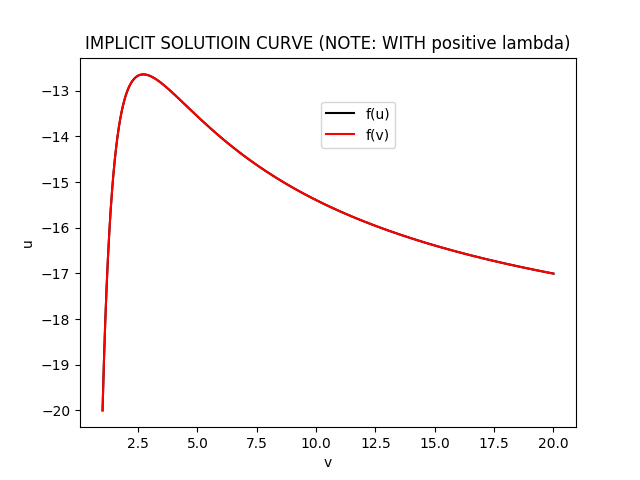
\includegraphics[width=\linewidth]{pos_lambda.png}
    \caption{u and v [$+\lambda$] }
  \end{subfigure}
\end{figure}

\pagebreak

\section*{Observation}
\textbf{We know that $v, u$ $\ge 0$ since we are dealing with population interaction. \\ \\ since $k$ is the intergral constant, we hence know that $k \in \Re$\\ \\ It is also given that $\lambda \in \Re$ or that $\lambda \in -\infty, \infty$ \\ \\ By using python i managed to see that, if $\lambda$ is negative($-\lambda$) then from Figure 1 it is evident that the implicit function is facing up and \\if $\lambda$ is positive($+\lambda$) then from Figure 2 it is evident that the implicit function is facing down. The change of the sign of $\lambda$ keeps the shape undeformed or unchanged but it changes the orientation of the implicit function with respect to the change in the sign of $\lambda$\\ \\ However, if we manipulate $k$ the shape of the implicit function remains undeformed(unchanged), but the implicit function is shifted up/ down relative to the the value of $k$}
\end{document}
